\documentclass[10pt]{exam}
\usepackage[phy]{template-for-exam}
\usepackage{tikz}
\usetikzlibrary{shadings,decorations.pathmorphing,arrows.meta}

\title{Simple Harmonic \#2}
\author{Rohrbach}
\date{\today}

\begin{document}
\maketitle

\begin{questions}
\question
  What are the two things that affect the period of a spring?
  \vs

\question
  Why does amplitude \emph{not} affect the period of a spring?
  \vs

\question
  Why \emph{does} mass affect the period of a spring?
  \vs

\question
  When an oscillating spring reaches the equilibrium position, the net restoring force is zero.  Why then does the spring continue to move past equilibrium and continue its oscillations?
  \vs


\question
  Where in the motion of a pendulum is the bob moving the fastest?  Why?
  
  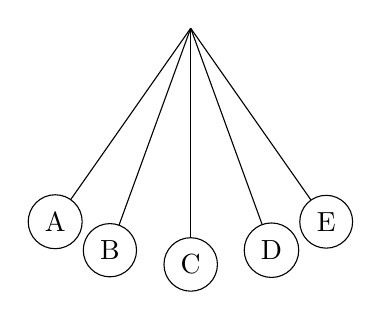
\begin{tikzpicture}[
    bob/.style={
      draw=black, fill=white, circle, radius=0.3
    }
  ]
    \draw (-125:3) node[bob] {A} -- (0,0);
    \draw (-110:3) node[bob] {B} -- (0,0);
    \draw (-90:3) node[bob] {C} -- (0,0);
    \draw (-70:3) node[bob] {D} -- (0,0);
    \draw (-55:3) node[bob] {E} -- (0,0);


  \end{tikzpicture}




\question
  A pinball machine uses a spring that is compressed {\bf 4.0~cm} to launch a ball.  If the spring constant is 13~N/m, what is the force on the ball at the moment the spring is released?
  \vs[2]



\pagebreak

\question
  Eddie wants to find the spring constant of a spring, so he hangs the spring vertically and attaches a 0.40-kg mass to the spring's end.  If the spring stretches {\bf 3.0~cm} from its equilibrium position, what is the spring constant?
  \vs

\question
  A spring with a spring constant of 30.0~N/m is attached to a 2.3~kg mass, and the system is set in motion.  Find the period and frequency.
  \vs

\question
  What mass must you attach to a spring of constant $k=103$~N/m in order for it to make 20 complete vibrations in 4.0~s?
  \vs[2]


\question 
  In the dark of night you are assigned the dubious task of determining the height of a tower upon which you will lay siege.  Conveniently, a pendulum is hanging from the tower to the ground.  If the pendulum has a period of 24~s, how tall is the tower?

  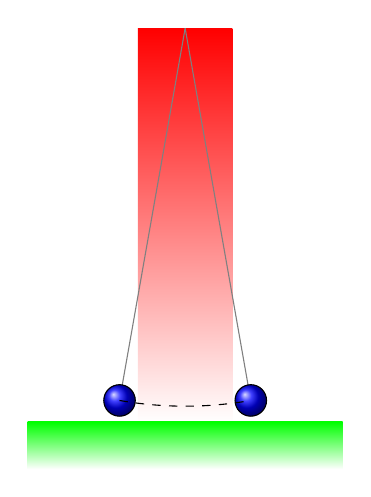
\begin{tikzpicture}
    \fill[top color=red] (-.6,0) rectangle (.6,-5);
    \fill[top color=green] (-2,-5) rectangle (2,-5.6);

    \draw[gray] (-100:4.8) -- (0,0);
    \draw[gray] (-80:4.8) -- (0,0);
    \filldraw[shading=ball] (-80:4.8) circle (0.2);
    \filldraw[shading=ball] (-100:4.8) circle (0.2);
    \draw[dashed] (-100:4.8) arc (-100:-80:4.8);

  \end{tikzpicture}


\end{questions}

\end{document}